\documentclass{article}

\usepackage{latexsym}
\usepackage{bbm}
\usepackage[small,bf]{caption2}
\usepackage{graphics}
\usepackage{epsfig}
\usepackage{amsmath,amssymb,amsthm,amsfonts}
\usepackage{url}
\usepackage{hyperref}
\usepackage{enumerate}

%% Page size
\setlength{\oddsidemargin}{0pt}
\setlength{\evensidemargin}{0pt}
\setlength{\textwidth}{6.5in}
\setlength{\topmargin}{0in}
\setlength{\textheight}{8.5in}

% Footnote commands.
\newcommand{\footnotenonumber}[1]{{\def\thempfn{}\footnotetext{#1}}}
\newcommand{\footnotetight}[1]{\footnote{\renewcommand\baselinestretch{1}\footnotesize #1}}

\newtheorem{propo}{Proposition}[section]
\newtheorem{lemma}[propo]{Lemma}
\newtheorem{definition}[propo]{Definition}
\newtheorem{coro}[propo]{Corollary}
\newtheorem{thm}[propo]{Theorem}
\newtheorem{conj}[propo]{Conjecture}
\newtheorem{fact}[propo]{Fact}
\newtheorem{remark}[propo]{Remark}
\newtheorem{claim}[propo]{Claim}

\newcommand{\T}{{\sf T}}
\newcommand{\Tk}{{\mathbb T_k^{\phi}}}
\newcommand{\Tl}{{\sf T(\ell)}}
\newcommand{\uH}{{\underbar{H}}}
\newcommand{\mulH}{{ \mu^{\ell,H}}}
\newcommand{\dTl}{{ \partial \T(\ell)}}
\newcommand{\bE}{\mathbb{E}}
\newcommand{\prob}{\mathbb{P}}
\newcommand{\IS}{{\rm IS}}
\newcommand{\ind}{\mathbb{I}}
\newcommand{\naturals}{\mathbb{N}}

\usepackage[numbib]{tocbibind}

\setlength{\parindent}{0pt}

\usepackage{framed}
\usepackage{color}
\definecolor{gray}{gray}{0.3}
\definecolor{darkgreen}{rgb}{0,0.55,0}
\definecolor{purple}{rgb}{0.5,0,1}

\newenvironment{comment}{
  \medskip
  \begin{framed}
    \bgroup\color{blue}
    {\textbf{Comment:}}
}{
\egroup\end{framed}
  \medskip
}

\begin{document}
    \section{Group DRO}
    In group DRO, assuming the training distribution $\hat{P}$ is a mix of group distributions $\hat{P_g}$ for $m$ groups $g \in \{ 1, 2, ..., m \}$. The intuitive DRO objective is
    \begin{align*}
        \hat{\theta}_{\text{DRO}} = \arg \min_{\theta \in \Theta} \sup_{g \in G} \mathbb{E}_{x, y \sim \hat{P_g}} [\ell(x, y, \theta)]
    \end{align*}

    The same problem can be rewritten as
    \begin{align*}
        \hat{\theta}_{\text{DRO}} = \arg \min_{\theta \in \Theta} \sup_{q \in \Delta m} \sum_{g=1}^{m} q_g \mathbb{E}_{x, y \sim \hat{P_g}} [\ell(x, y, \theta)]
    \end{align*}
    where $q$ can be viewed as a weight distribution for each group distribution. In realization, $q$ will have 1 on the group with the worst group loss which simulates the original formulation of the problem. Otherwise, the supremum will not be satisfied.

    \section{Noisy Group Attributes}
    Now, we are interested in problems where our empirical group distribution is noisy. Consider an empirical distribution $\hat{P}$ made of a mix of two true group distributions $\hat{P_1}$ and $\hat{P_2}$. However, we don't have access to these two true group distributions. Instead, we have access to $\tilde{P_1}$ and $\tilde{P_2}$ where some samples in $\tilde{P_1}$ and $\tilde{P_2}$ are misclassified. Suppose the error rate for the group information is $\epsilon_1$ and $\epsilon_2$. In other words, samples that are truly in group 1 can be categorized into group 2 with probability of $\epsilon_1$ and samples that are truly in group 2 can be categorized into group 1 with probability of $\epsilon_2$. Thus, we can represent 
    \begin{align*}
        \tilde{P_1} &= \frac{\prob[G = 1] \cdot (1 - \epsilon_1)}{\prob[G = 1] \cdot (1 - \epsilon_1) + \prob[G = 2] \cdot \epsilon_2} \hat{P_1} + \frac{\prob[G = 2] \cdot \epsilon_2}{\prob[G = 1] \cdot (1 - \epsilon_1) + \prob[G = 2] \cdot \epsilon_2} \hat{P_2}
        \\ \tilde{P_2} &= \frac{\prob[G = 1] \cdot \epsilon_1}{\prob[G = 1] \cdot \epsilon_1 + \prob[G = 2] \cdot (1 - \epsilon_2)} \hat{P_1} + \frac{\prob[G = 2] \cdot (1 - \epsilon_2)}{\prob[G = 1] \cdot \epsilon_1 + \prob[G = 2] \cdot (1 - \epsilon_2)} \hat{P_2}
    \end{align*}

    For notation simplicity, we let
    \begin{align*}
        \alpha_1 &= \frac{\prob[G = 1] \cdot (1 - \epsilon_1)}{\prob[G = 1] \cdot (1 - \epsilon_1) + \prob[G = 2] \cdot \epsilon_2}
        \\ \alpha_2 &= \frac{\prob[G = 1] \cdot \epsilon_1}{\prob[G = 1] \cdot \epsilon_1 + \prob[G = 2] \cdot (1 - \epsilon_2)}
    \end{align*}

    Then,
    \begin{align*}
        \tilde{P_1} &= \alpha_1 \cdot \hat{P_1} + (1 - \alpha_1) \cdot \hat{P_2}
        \\ \tilde{P_2} &= \alpha_2 \cdot \hat{P_1} + (1 - \alpha_2) \cdot \hat{P_2}
    \end{align*}

    In the context of Group DRO, with access to the true group distributions, we want to optimize
    \begin{align*}
        \hat{\theta}_{\text{DRO}} = \arg \min_{\theta \in \Theta} \sup_{q \in \Delta m} q_1 \mathbb{E}_{x, y \sim \hat{P_1}} [\ell(x, y, \theta)] + q_2 \mathbb{E}_{x, y \sim \hat{P_2}} [\ell(x, y, \theta)]
    \end{align*}

    If we naively use Group DRO on the noisy group distributions $\tilde{P_1}, \tilde{P_2}$, we are actually solving
    \begin{align*}
        \tilde{\theta}_{\text{DRO}} &= \arg \min_{\theta \in \Theta} \sup_{\tilde{q} \in \Delta m} \tilde{q_1} \mathbb{E}_{x, y \sim \tilde{P_1}} [\ell(x, y, \theta)] + \tilde{q_2} \mathbb{E}_{x, y \sim \tilde{P_2}} [\ell(x, y, \theta)]
        \\ &= \arg \min_{\theta \in \Theta} \sup_{\tilde{q} \in \Delta m} (\tilde{q_1} \alpha_1 + \tilde{q_2} \alpha_2) \mathbb{E}_{x, y \sim \hat{P_1}} [\ell(x, y, \theta)] + (\tilde{q_1} (1-\alpha_1) + \tilde{q_2} (1 - \alpha_2)) \mathbb{E}_{x, y \sim \hat{P_2}} [\ell(x, y, \theta)]
    \end{align*}

    \begin{comment}
        This above equation seems to make sense but also not really. Ignoring the minimization problem outside, if we focus on the supremum inside, we see that the first one should achieve a $\tilde{q}^\ast$ s.t. a weight of 1 is put on the maximum between $\mathbb{E}_{x, y \sim \tilde{P_1}} [\ell(x, y, \theta)]$ and $\mathbb{E}_{x, y \sim \tilde{P_2}} [\ell(x, y, \theta)]$. However, taking a look at the second equation, the ideal solution for the supremum should achieve $\tilde{q}^\ast$ s.t. either $(\tilde{q_1} \alpha_1 + \tilde{q_2} \alpha_2)$ or $(\tilde{q_1} (1-\alpha_1) + \tilde{q_2} (1 - \alpha_2))$ achieves is 1 depending on the maximum between $\mathbb{E}_{x, y \sim \hat{P_1}} [\ell(x, y, \theta)]$ and $\mathbb{E}_{x, y \sim \hat{P_2}} [\ell(x, y, \theta)]$
    \end{comment}

    We can make some observations
    \begin{enumerate}
        \item For a given $\tilde{q}$ when optimizing for $\tilde{\theta}_{\text{DRO}}$ using the noisy group distributions, we are actually using a transformed $q$ in optimizing with non-noisy group distributions. For instance, if we at some point $\tilde{q_1} = t$ and $\tilde{q_2} = 1 - t$ in the context of noisy group distributions, it's actually representing $q_1 = t \cdot \alpha_1 + (1-t) \cdot \alpha_2$ and $q_2 = t \cdot (1 - \alpha_1) \cdot (1-t) \cdot (1 - \alpha_2)$ in optimizing with true group distributions. 
        \item With the transformation, searching in the space of $\Delta m$ for $q$ and $\tilde{q}$ are different because $\tilde{q}$ in $\Delta m$ does not correspond to the same space $\Delta m$ for $q$.
        \item The transformation can be written as
        \begin{align*}
            \begin{bmatrix}
                q_1 \\ q_2
            \end{bmatrix} = \begin{bmatrix}
                \alpha_1 & \alpha_2
                \\ 1 - \alpha_1 & 1 - \alpha_2
            \end{bmatrix} \begin{bmatrix}
                \tilde{q_1} \\ \tilde{q_2}
            \end{bmatrix}
        \end{align*}

        So if we know $\Delta m$ contains the $q$ we are interested in, then 
        \begin{align*}
            \tilde{\Delta m} &= \begin{bmatrix}
                \alpha_1 & \alpha_2
                \\ 1 - \alpha_1 & 1 - \alpha_2
            \end{bmatrix}^{-1} \Delta m
        \end{align*}
        would contain the corresponding $\tilde{q}$.
        \item When $\epsilon_1 = \epsilon_2 = 0$, the objective is the same for original group DRO with the true group distributions because $\alpha_1 = 1$ and $\alpha_2 = 0$ form an identity matrix.
    \end{enumerate}

    \section{Online Group DRO}
    \begin{center}
        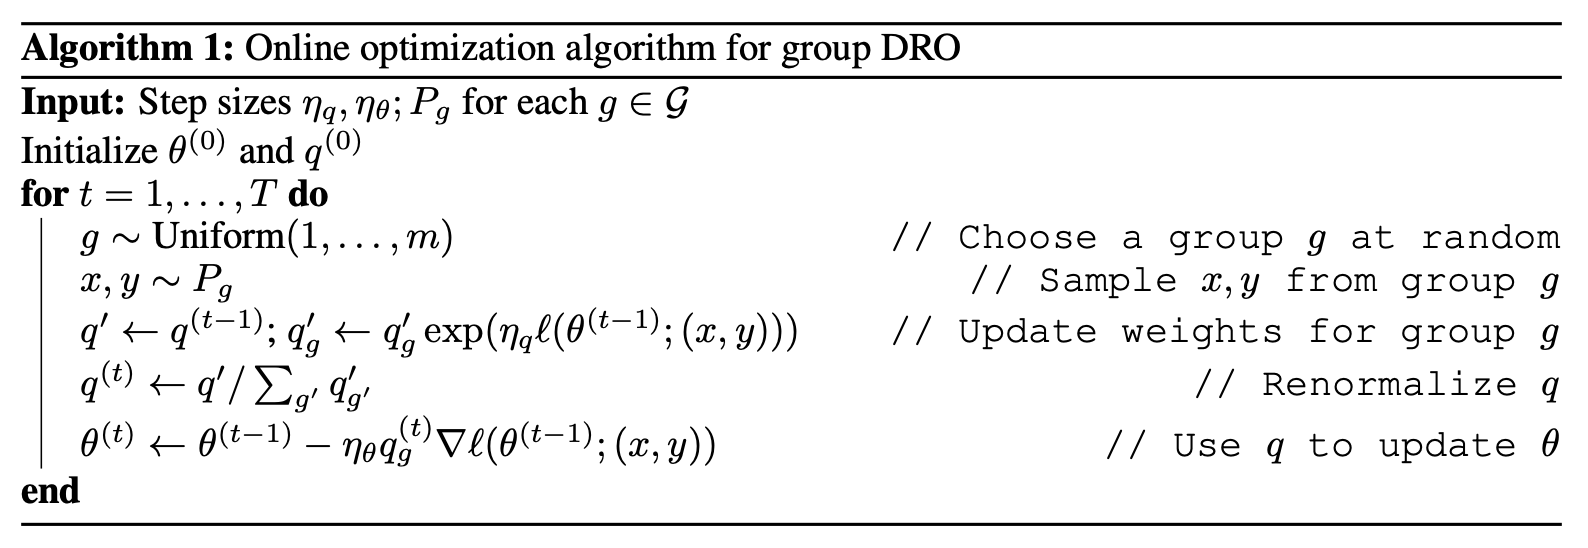
\includegraphics[scale=0.5]{online_group_dro.png}
    \end{center}

    \section{Bound error rate}
    % Let $H = \begin{bmatrix}
    %     \alpha_1 & \alpha_2 
    %     \\ 1 - \alpha_1 & 1 - \alpha_2
    % \end{bmatrix}$. As aforementioned, in the ideal solution, either $q_1 = 1$ or $q_2 = 1$. In the case of $q_1 = 1$, when we perfectly optimize $\tilde{q_1}, \tilde{q_2}$ s.t. either $\tilde{q_1} = 1$ or $\tilde{q_2} = 1$, we can analyze the two cases
    % \begin{enumerate}
    %     \item $\tilde{q_1} = 1$
    % \end{enumerate}

    \bibliographystyle{plain} % We choose the "plain" reference style
    \bibliography{refs} % Entries are in the refs.bib file
\end{document}